% !TeX root = ../main.tex

\section*{Hidden Markov Models HMM}
\paragraph{Idea:}  A HMM \(\lambda = (A, B, \vec{\pi})\) is a generative\footnote{models the joint probability $p(<o_1,\dots, o_M>, <S_1,\dots, S_M>)$ of hidden states and a sequence} probabilistic approach to describing sequential data (e.g. speech data).

\begin{itemize}
	\item A is a matrix of state transition probabilities \(a_{ij} = P[q_{t+1} = S_j | q_t = S_i]\)
	\item B is a matrix of production probabilities \(b_j(v_k) = P[v_k at state S_j]\), where \(V={v_1,\dots,v_{|V|}}\) is the set of possible observations.
	\item Values in each row of the matrices A and B sum up to 1.
	\item \(\vec{\pi}\) is a vector of starting probabilities for each state.
\end{itemize}

\begin{figure}[H]
	\centering
	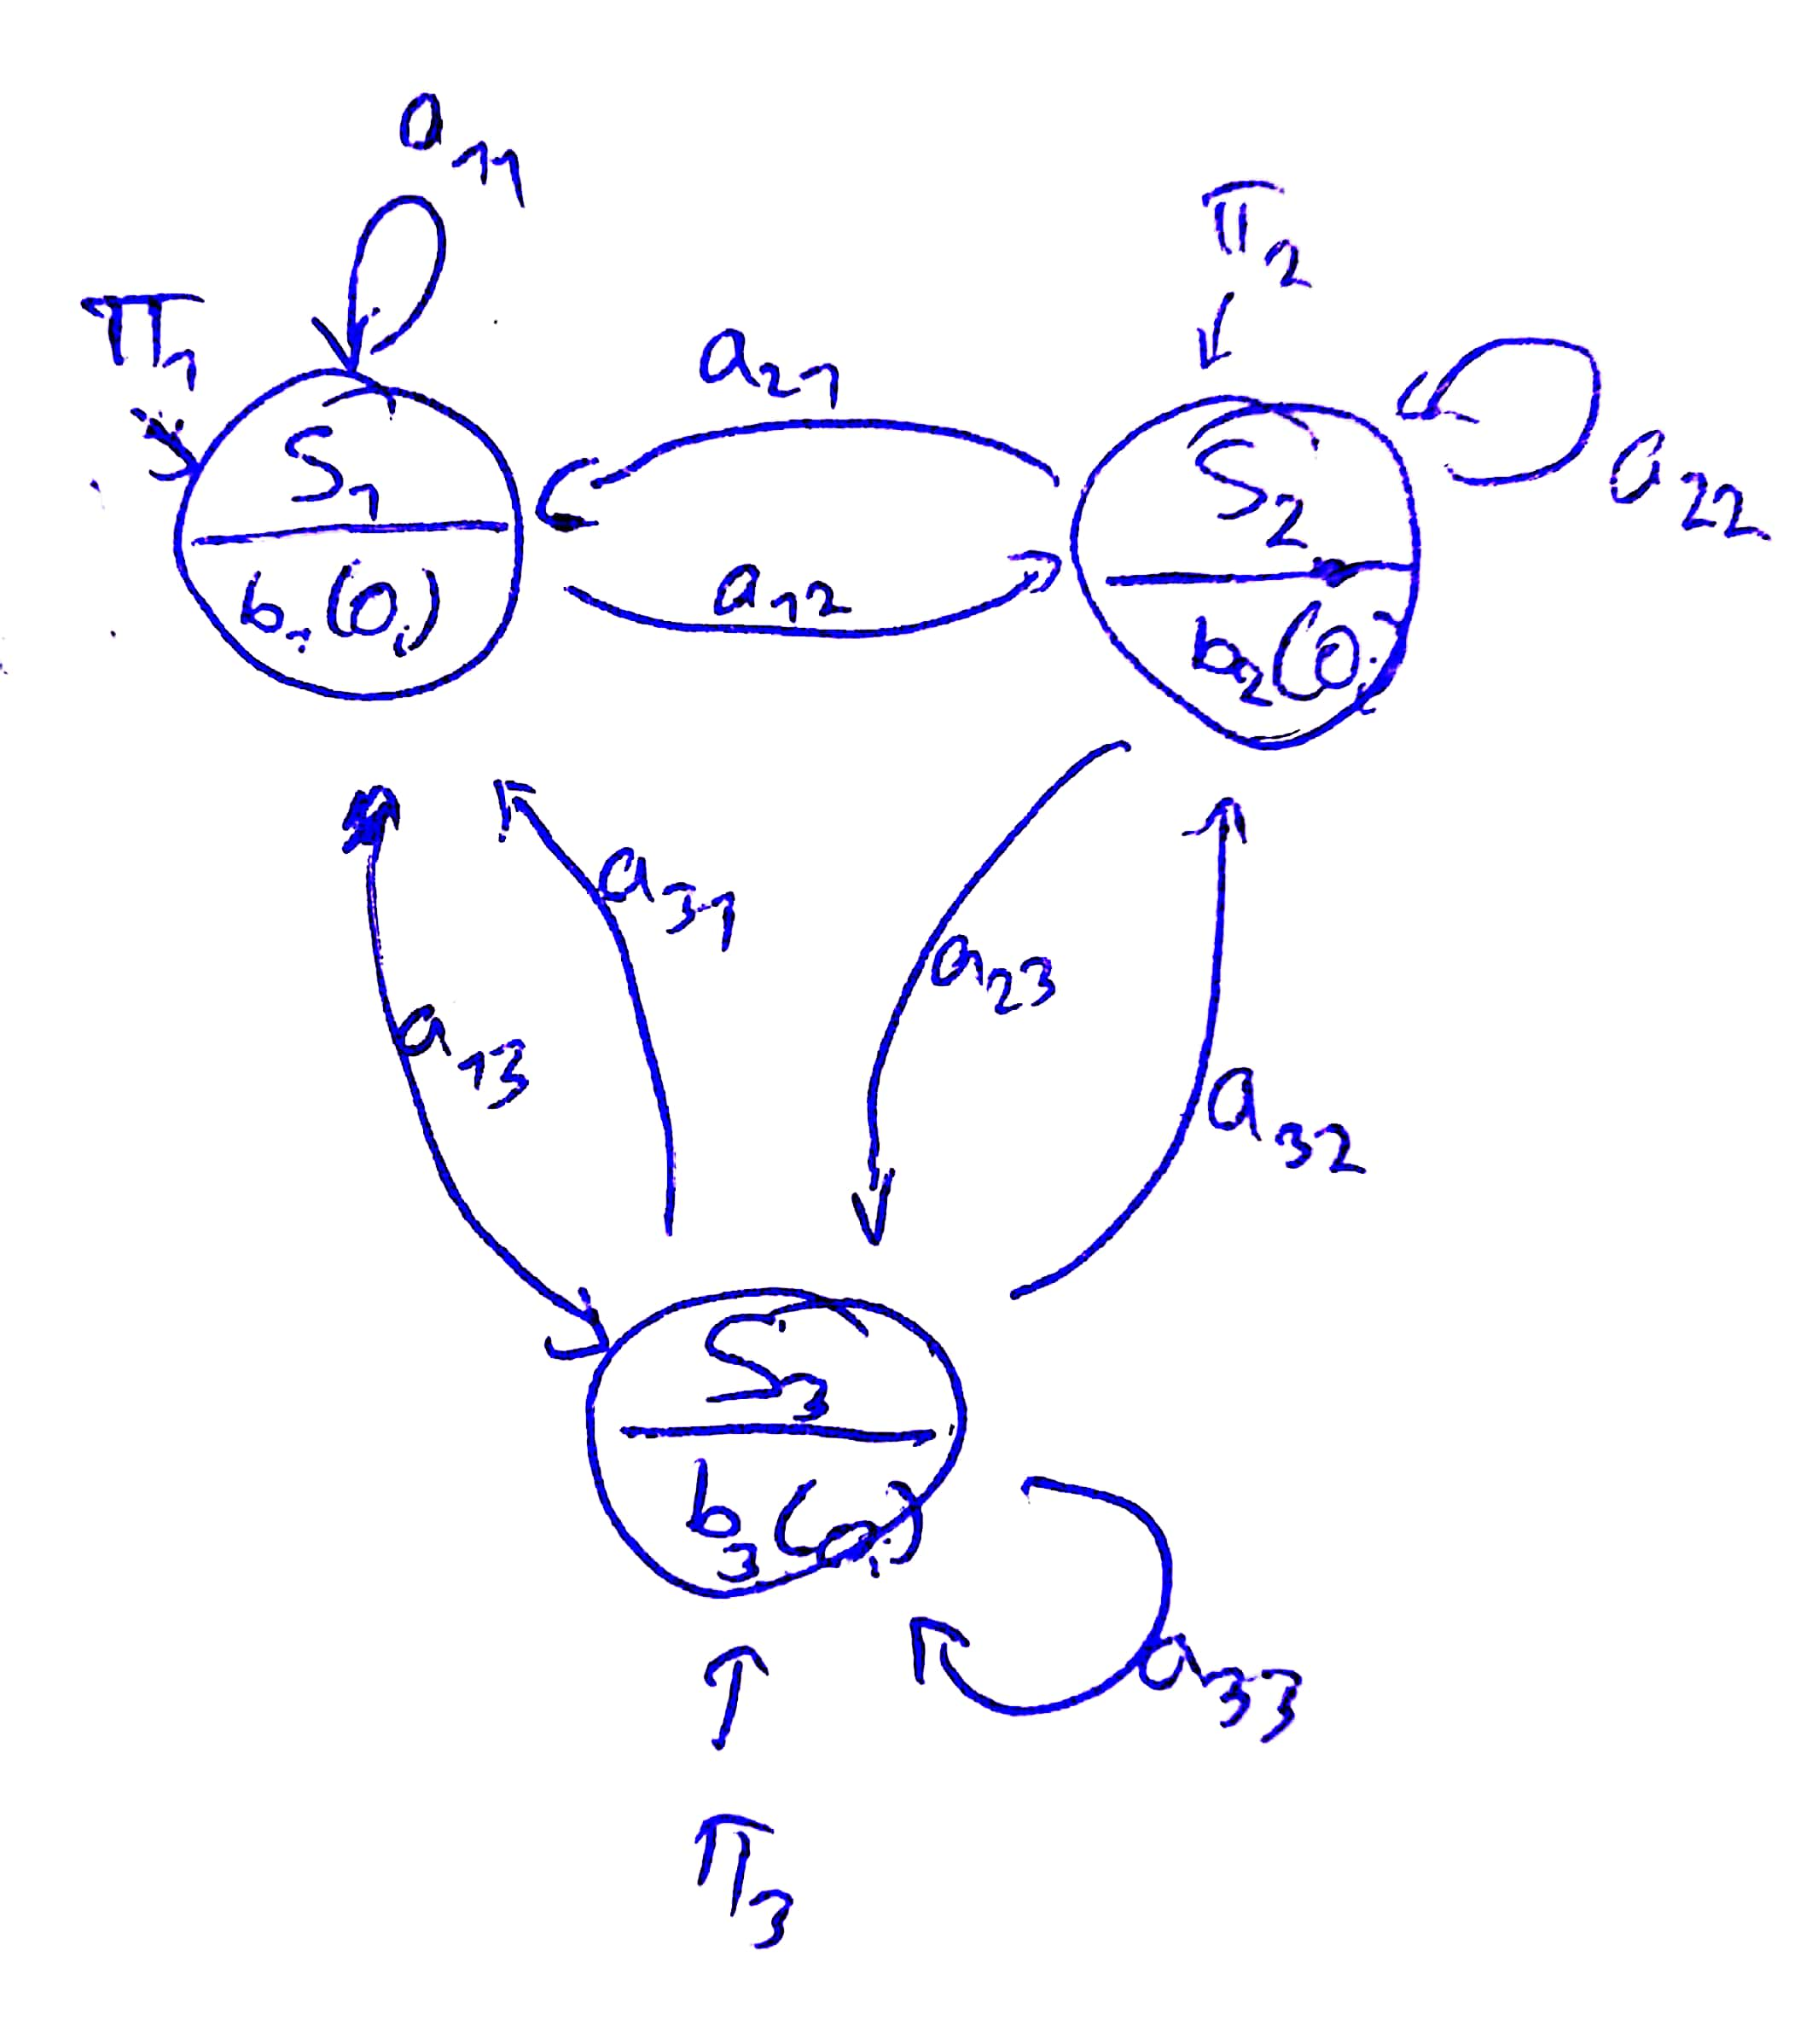
\includegraphics[width=0.4\textwidth]{hmm.jpg}
	\caption{We can represent a HMM as a graphical model similar to a state machine.}
\end{figure}



\subsection*{Production probability of an observation: \emph{Forward-/Backward-Algorithm}}
Given a model \(\lambda\), what is \(p(<o_1,\dots, o_M>|\lambda)\), the probability of making an observation \(<o_1,\dots, o_M>\) given \(\lambda\)?

Simple idea: Marginalize over all state sequences \footnote{The sums enumerate all possible state sequences; The products represent \(p(<S_1,\dots,S_M>) \cdot (p(<o_1,\dots, o_M>|<S_1,\dots,S_M>)\)}:

\[p(<o_1,\dots,o_M>|\lambda) = \sum_{S_1=1}^{N} \sum_{S_2=1}^{N} \dots \sum_{S_M=1}^{N} \pi_{S_1} \cdot \prod_{i=1}^{M-1} a_{S_i S_{i+1}} \cdot \prod_{i=1}^{M} b_{S_i}(o_i)\]

Problems with implementation:
\begin{itemize}
	\item Computing cost: \(O(N^M)\), because the sums will create M for loops
	% \item Multiplying many small values will cause precision problems
	\item Solution: dynamic programming (compute each factor as rarely / early as possible) $\Rightarrow$ Forward-/Backward Algorithm
	\[p(<o_1,\dots,o_M>|\lambda) = \sum_{S_1=1}^{N} \pi_{S_1} b_{S_1}(o_1) \cdot \sum_{S_2=1}^{N} a_{S_1 S_2} b_{S_2}(o_2) \cdot \quad \ldots \quad \cdot \sum_{S_M=1}^{N} a_{S_{M - 1} S_{M}} b_{S_M}(o_M)\]
\end{itemize}

\paragraph{Forward Algorithm:}

\begin{enumerate}
    \item Initialization:
        \(\alpha_1(i) = \pi_i b_i(o_1)\)
    \item Induction:
        \(\alpha_{t+1}(j) = (\sum_{i=1}^N \alpha_t(i) \cdot a_{ij}) b_j(o_{t+1})\)
    \item Termination:
        \(P(O|\lambda) = \sum_{i=1}^N \alpha_T(i)\)
\end{enumerate}

Meaning of $\alpha_t(i)$: Sum of all paths (probabilities) to end up in state $i$ in time step $t$.

\begin{figure}[H]
	\centering
	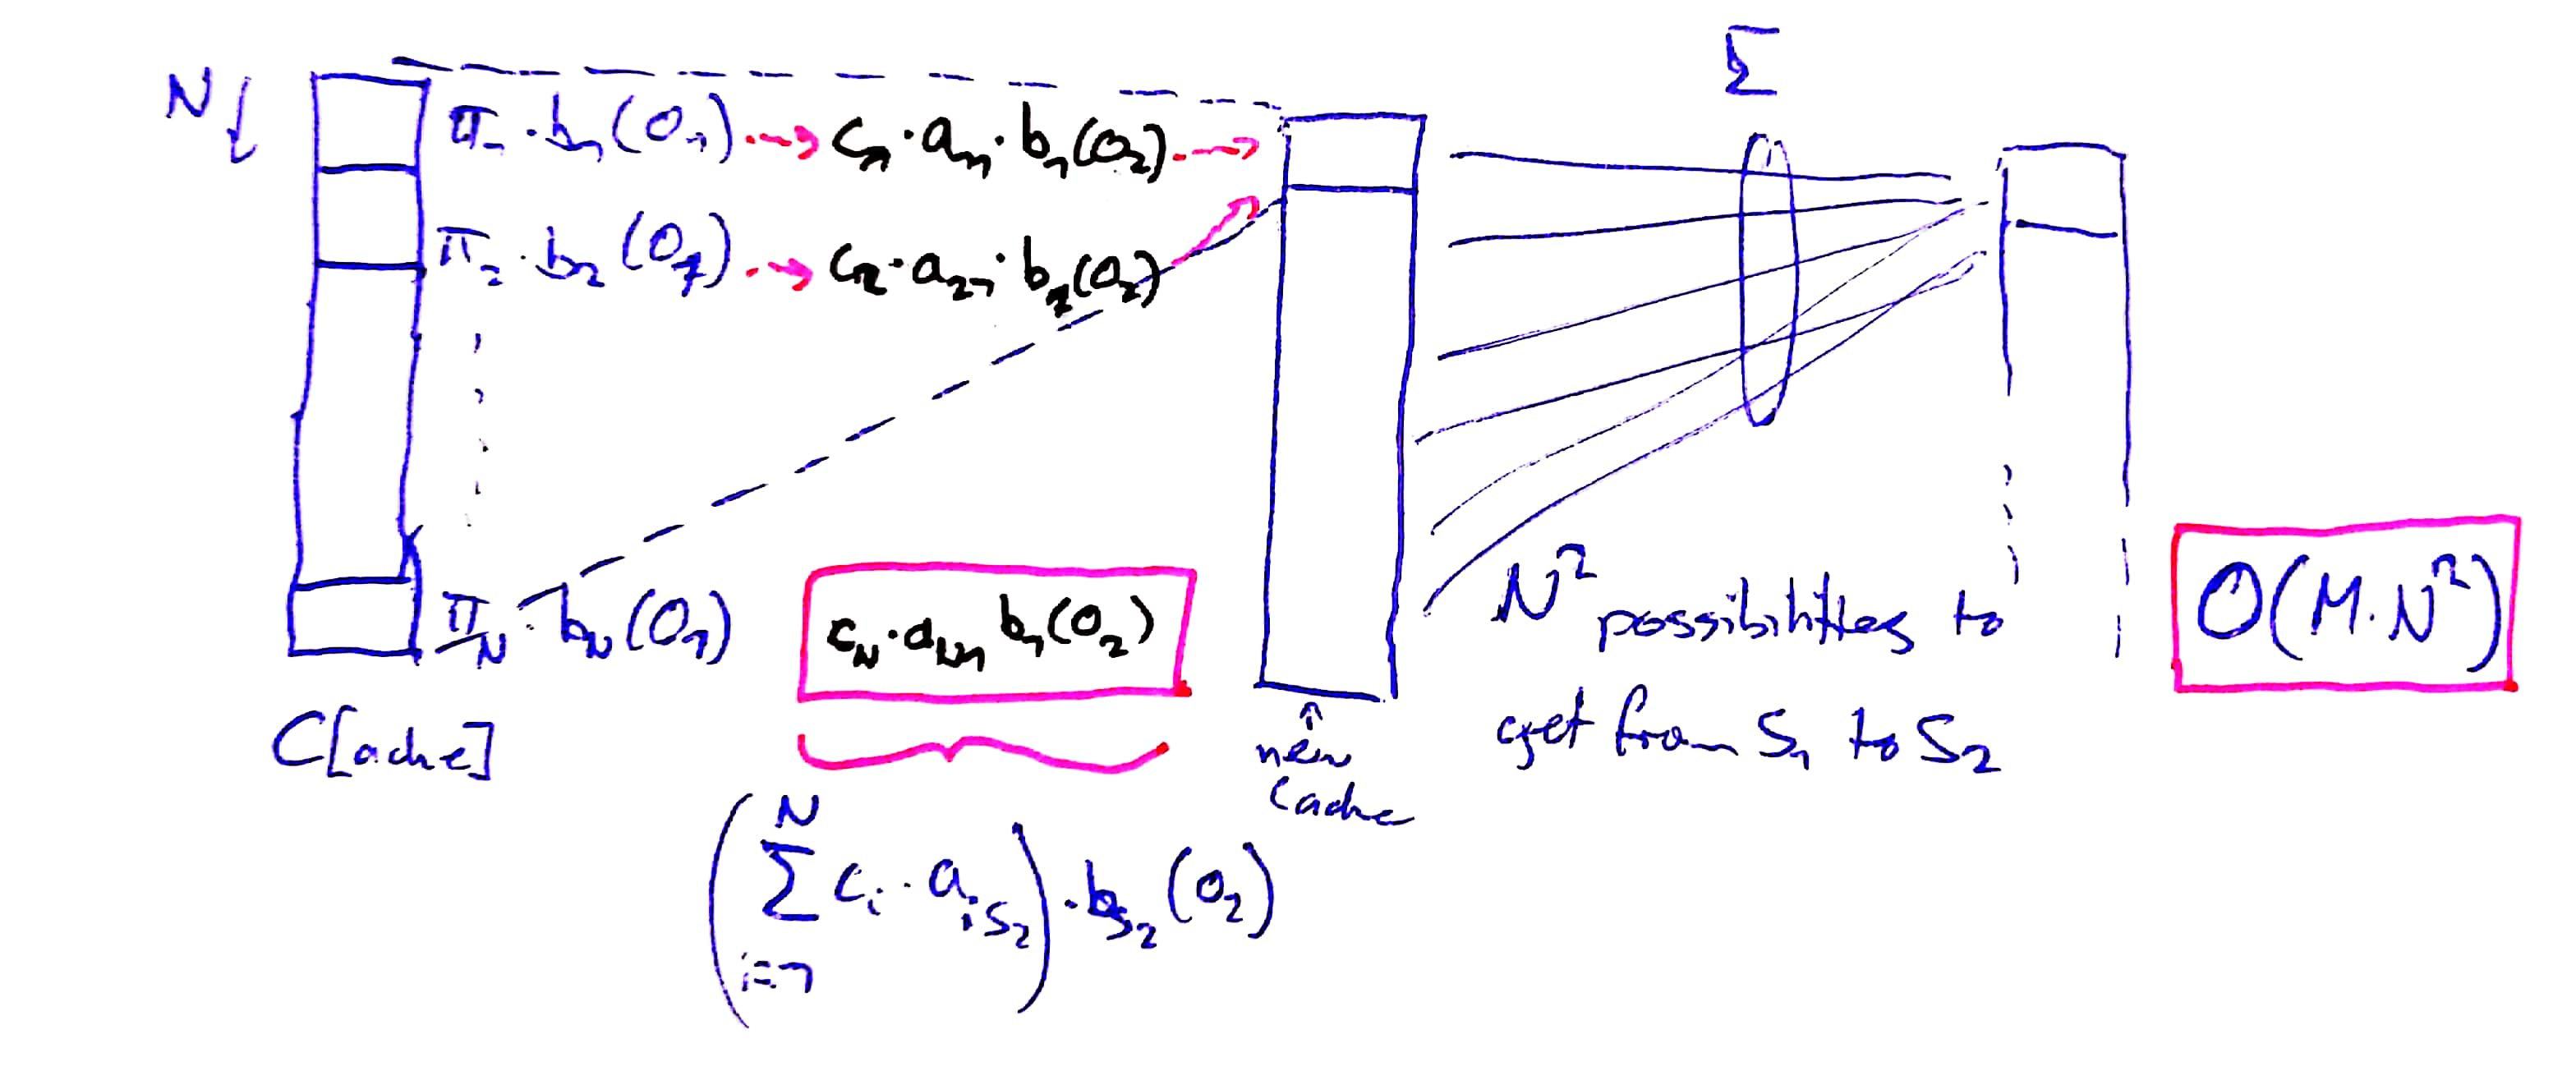
\includegraphics[width=0.9\textwidth]{forward.jpg}
\end{figure}

\paragraph{Backward Algorithm:}

\begin{enumerate}
    \item Initialization: \(\beta_T (i) = 1\) (choosen arbitrarily)
    \item Induction: \(\beta_t(i) = \sum_{j=1}^N a_{ij} b_j(o_{t+1}) \beta_{t+1}(j)\)
\end{enumerate}

Meaning of $\beta_t(i)$: integration of all future paths (probabilities).

\begin{figure}[H]
  \centering
  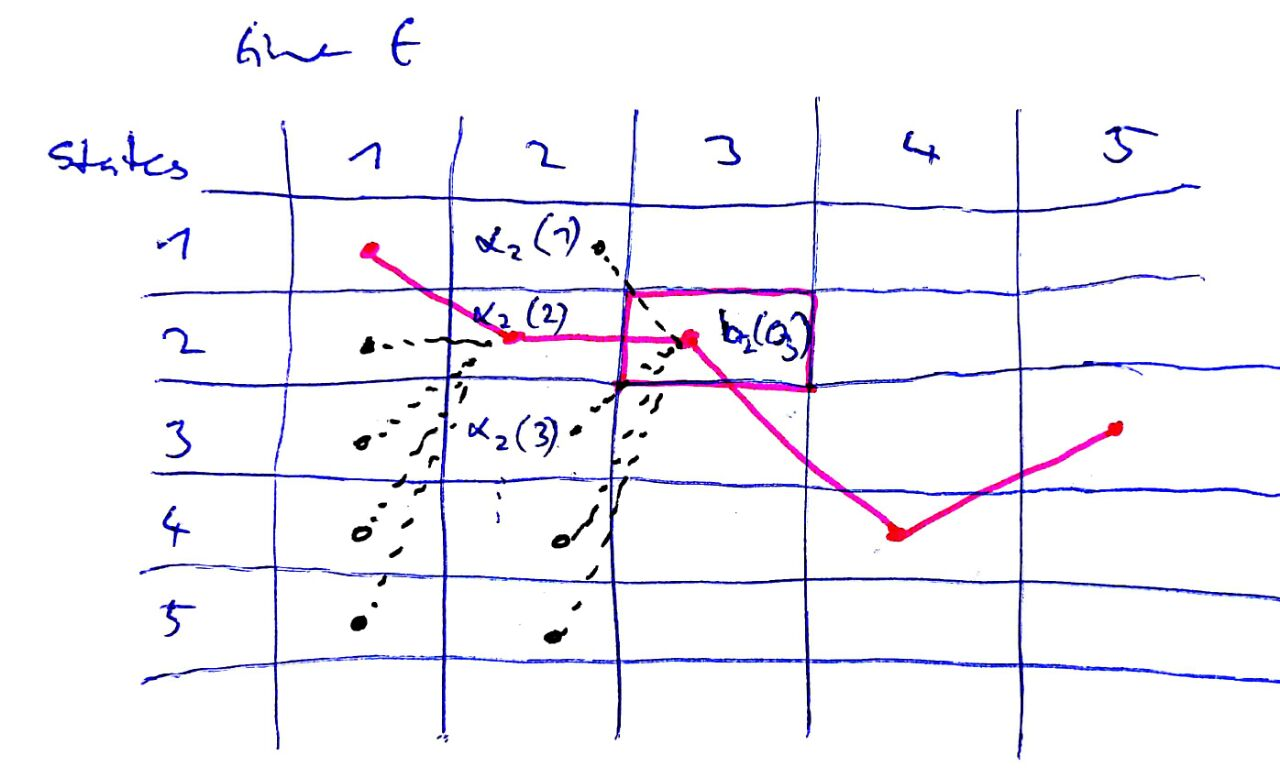
\includegraphics[width=0.7\textwidth]{backward}
\end{figure}

\subsection*{Most likely state sequence: \emph{Viterbi Algorithm}}

Given a model \(\lambda\) and an observation sequence \(<o_1,\dots, o_M>\), what is the most likely sequence of states \(<S_1,\dots, S_M>\) that generated it?

Naive idea: Choose the most likely state at each time step $t$. But the resulting state sequence may not make sense as a whole.

Solution: Choose the best state sequence Q with the highest $\delta_t(i) = \max_{Q_1, \ldots, Q_{t-1}} P[q_1, \ldots, q_t=i, o_1, \ldots, q_t | \lambda]$, that ends at the time step $t$ in state $S_i$.

\paragraph{Viterbi Algorithm:}

\begin{enumerate}
    \item Initialization:
        \begin{align*}
            \delta_1(i) &= \pi_i b_i(O_1)\\
            \psi_1(i) &= 0
        \end{align*}
    \item Recursion:
        \begin{align*}
            \delta_t(j) &= \max_i (\delta_{t-1}(i) \alpha_{ij} \cdot b_j(O_{t+1}))\\
            \psi_t(j) &= \argmax_i (\delta_{t-1}(i) \alpha_{ij})
        \end{align*}
				, where $\psi_t(i)$ holds the index of the previous most likely state sequence in $\delta_{t-1}(i)$.
    \item Termination:
        \begin{align*}
            P^* &= \max_i \delta_T(i)\\
            q_T^* &= \argmax_i \delta_T(i)
        \end{align*}
    \item Path (state sequence) backtracking:
        \[q_t^* = \psi_{t+1}(q_{t+1}^*), \qquad \text{for } t = T-1, \dots, 1\]
\end{enumerate}


\subsection*{Training of a HMM: \emph{Baum-Welch-Algorithm}}

How can we obtain the model parameters \(\lambda = (A, B, \vec{\pi})\) in a fully automated way (training)?

Solution: Choose \(\lambda = (A, B, \vec{\pi})\) to locally maximize $p(O|\lambda)$

\paragraph{Auxiliary Variables}
\begin{itemize}
	\item $\alpha_t(i) = p(o_1,\dots, o_t, q_t=S_i|\lambda)$: probability of partial observation sequence ending in $S_i$ at time $t$.
	\item $\beta_t(i) = p(o_1,\dots, o_t | q_t=S_i, \lambda)$: probability of partial future observation sequence starting in $S_i$ at time $t$.
	\item $\gamma_t(j) = p(q_t=S_i|O, \lambda)$: probability of being in state $S_j$ at time $t$.
	\item $\xi_t(i,j) = p(q_t=S_i, q_{t+1}=S_j|O, \lambda)$: probabiltiy of transitioning from $S_i$ to $S_j$ at time $t$.
\end{itemize}

\paragraph{Baum-Welch-Algorithm (EM-type Algorithm):}

\begin{enumerate}
    \item Initialization: \(\lambda = (A, B, \vec{\pi})\)
    \item While ($\bar{\lambda} \neq \lambda$) {
		\begin{enumerate}
			\item $\lambda = \bar{\lambda}$
			\item \textbf{E-Step:} update $\alpha, \beta, \gamma, \xi$
			\item \textbf{M-Step:}
			\begin{align*}
				\bar{\pi}_i &= \gamma_1(i) \\
				\bar{a}_{i,j} &= \dfrac{\sum_{t=1}^{T-1} \xi_t(i,j)}{\sum_{t=1}^{T-1} \gamma_t(i)} = \dfrac{\text{expected \# of transitions from} \ S_i \rightarrow S_j}{\text{expected \# of transitions from} \ S_i} \\
				\bar{b}_{j}(k) &= \dfrac{\sum_{t=1 \text{ if } o_t=v_k}^{T} \gamma_t(i)}{\sum_{t=1}^{T} \gamma_t(i)} = \dfrac{\text{expected \# of times in }S_j \text{with symbol }v_k}{\text{expected \# of times in} \ S_j} \\
				\bar{\lambda} &= (\bar{A}, \bar{B}, \bar{\vec{\pi}})
			\end{align*}
		\end{enumerate}
		}
\end{enumerate}



\subsection*{Remarks on HMM}

\begin{itemize}
    \item the directed edge in a HMM graph can be understood as a statistical dependency $p(S_2|S_1)$
    \item generative approch
    \item For many tasks including speach processing, we often only allow state transitions $a_{ij}$ with $i \le j$ (no backward links). So called "left-right-HMMs".
\end{itemize}
